\section{Results}

\subsection{Impulse Resonse Function}


\begin{figure}
    \centering
    \begin{minipage}{0.48\textwidth}
        \centering
        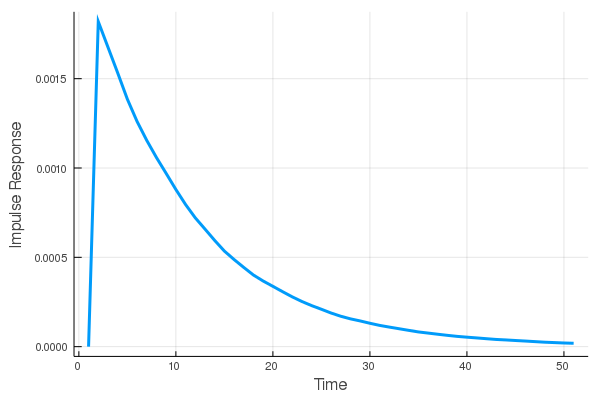
\includegraphics[width = \textwidth]{../tasks/Golosov_lucas/output/C_irf_50_periods.png}
        \caption{IRF till 50 periods after the shock}
        \label{irf1}
    \end{minipage}
    \begin{minipage}{0.48\textwidth}
        \centering
        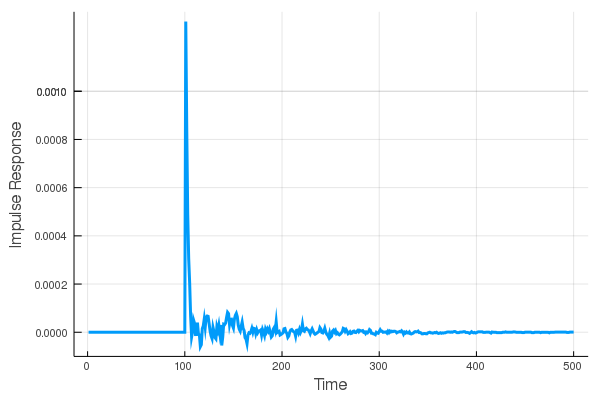
\includegraphics[width=\textwidth]{../tasks/Golosov_lucas/output/C_irf_500_periods.png}
        \caption{IRF for the entire simulation}
        \label{irf2}
    \end{minipage}
\end{figure}

On doubling the menu cost from 0.045 to 0.09 the variance of output increase by 3.038 times. Output IRF on impact is 98.5 percent.

\begin{figure}
    \centering
    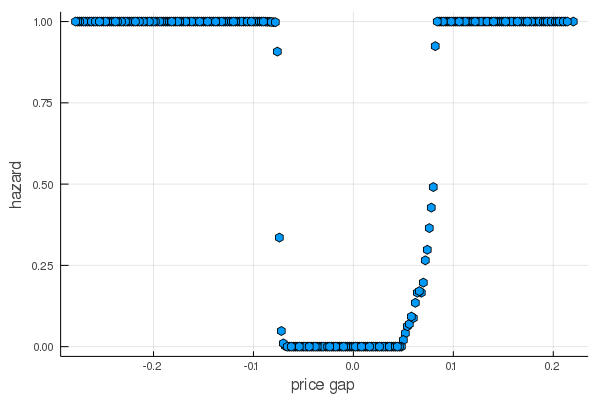
\includegraphics[width = 0.6\textwidth]{../tasks/Golosov_lucas/output/hazard_gl.png}
    \caption{Hazard}
    \label{}
\end{figure}

\begin{figure}
    \centering
    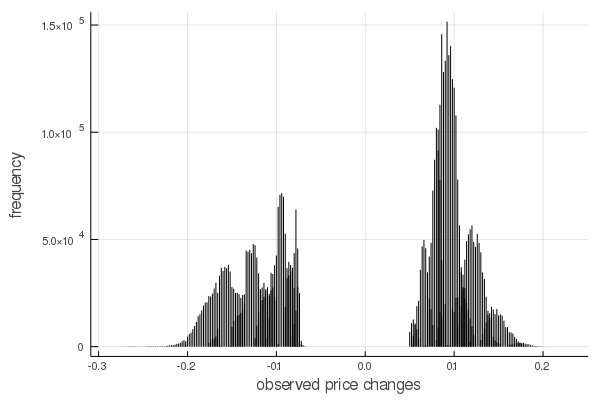
\includegraphics[width = 0.6\textwidth]{../tasks/Golosov_lucas/output/observed_p_changes_gl.png}
    \caption{Observed Price Changes}
    \label{}
\end{figure}

\begin{figure}
    \centering
    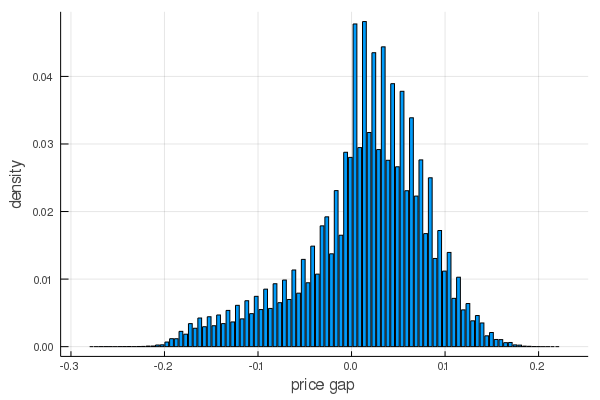
\includegraphics[width = 0.6\textwidth]{../tasks/Golosov_lucas/output/price_gap_dist.png}
    \caption{Price Gap Distribution}
    \label{}
\end{figure}
